\documentclass[8pt]{article}

\usepackage{fullpage}
\usepackage{tikz}
\usepackage[a4paper,bindingoffset=0.2in,%
            left=1in,right=1in,top=1in,bottom=1in,%
            footskip=.25in]{geometry}
\usetikzlibrary{shapes.geometric, arrows}
\tikzstyle{startstop} = [rectangle, rounded corners, minimum height=0.5cm,text centered, draw=black, fill=red!30]
\tikzstyle{io} = [trapezium, trapezium left angle=70, trapezium right angle=110, minimum height=0.8cm, text centered, draw=black, fill=blue!30]
\tikzstyle{process} = [rectangle, minimum width=1cm, minimum height=1cm, text centered, draw=black, fill=orange!30]
\tikzstyle{decision} = [diamond, minimum width=1cm, minimum height=1cm, text centered, draw=black, fill=green!30]
\tikzstyle{arrow} = [thick,->,>=stealth]    
\tikzstyle{line} = [thick,-,>=stealth] 

\begin{document}

\title{ARM Final Report}
\author{Fawwaz Abdullah (ffa20), Robert Buxton (rb419), \\Edward Hartley (ech120), Wojtek Sowinski (ws420) }

\maketitle

\section{ARM implementation}

 
\subsection{Assembler Data Structures}

\begin{itemize}

    \item \textbf{Map} (\texttt{StringUintMap}) A map implemented using an
    red-black tree and hashing function to allow strings to be mapped to unsigned
    32 bit intergers. This is used in two cases. Firstly to map branch tags to 
    memory locations and secondly to translate assembly inputs to their respective
    enum representations to be parsed. The root (a MapNode) and number of nodes is stored.
    
    \item \textbf{Tree Node} (\texttt{MapNode}) A node in the red-black tree that 
    stores the hash identifier of the node, the number of symbols with this hash, 
    a list of symbols (\_\_StringUintPair\_\_), the colour of the node which is used for balancing, the 
    parent node, and the left and right children.

    \item \textbf{Symbol Pair} (\texttt{\_\_StringUintPair\_\_}) a strut holding a
    string (identifier of the symbol) and a corresponding value (either an 
    address or enum value). 

    
    \item \textbf{Query Result} (\texttt{QueryResult}) a strut returned when searching the map
    holding the if a result was found and what it is if it was.
    
    \end{itemize}

\begin{minipage}{0.45\textwidth}
\subsection{Emulator Program Structure}

\begin{itemize}
    \item \texttt{parser.c} \\Contains the function that collects the symbols in the first pass of the
    input data and resets the file to be reread for the second pass
    \item \texttt{symbols.c} \\Contains the functions that create and interact with the
    symbol map used to map labels to memory addresses.
    \item \texttt{assemble.c} \\Initalises the maps used in the assembler. Then 
    passes over the file twice mapping labels to memory addresses and converting
    instructions into binary.
    \item \texttt{branch.c} \\Handles converting the branch instruction
    \item \texttt{dataprocessing.c} \\Handles converting the data processing
    instructions
    \item \texttt{multiply.c} \\Handles the multiply instructions
    \item \texttt{singledatatransfer.c} \\Handles the single data transfer instructions
\end{itemize}
\end{minipage}%
\hfill
\begin{minipage}{0.45\textwidth}

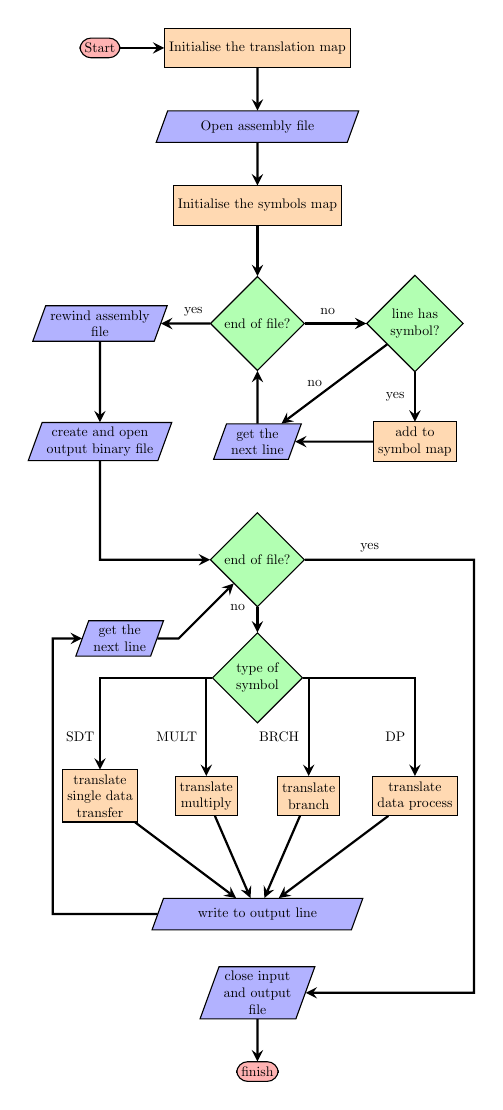
\begin{tikzpicture}[node distance=2cm]
    \node (start) [scale=0.5, startstop, align=center] at (0,0) {Start};
    \node (init_map) [scale=0.5, process, align=center] at (2,0) {Initialise the translation map};
    \node (open_file) [scale=0.5, io, align=center] at (2,-1) {Open assembly file};
    \node (init_map2) [scale=0.5, process, align=center] at (2,-2) {Initialise the symbols map};
    \node (end_file?) [scale=0.5, decision, align=center] at (2,-3.5) {end of file?};
    \node (is_symbol) [scale=0.5, decision, align=center] at (4,-3.5) {line has \\ symbol?};
    \node (add_map) [scale=0.5, process, align=center] at (4,-5) {add to \\ symbol map};
    \node (get_line) [scale=0.5, io, align=center] at (2,-5) {get the \\ next line};
    \node (rewind) [scale=0.5, io, align=center] at (0,-3.5) {rewind assembly \\ file};
    \node (create_file) [scale=0.5, io, align=center] at (0,-5) {create and open \\ output binary file};
    \node (end_file?2) [scale=0.5, decision, align=center] at (2,-6.5) {end of file?};
    \node (symbol_type) [scale=0.5, decision, align=center] at (2,-8) {type of \\ symbol};
    \node (sdt) [scale=0.5, align=center, process] at (0,-9.5) {translate \\ single data \\ transfer };
    \node (mult) [scale=0.5, align=center, process] at (1.35,-9.5) {translate \\ multiply};
    \node (brch) [scale=0.5, align=center, process] at (2.65,-9.5) {translate \\ branch};
    \node (dp) [scale=0.5, align=center, process] at (4,-9.5) {translate \\ data process};
    \node (write_out) [scale=0.5, io, align=center] at (2,-11) {write to output line};
    \node (get_line2) [scale=0.5, io, align=center] at (0.25,-7.5) {get the \\ next line};
    \node (close) [scale=0.5, io, align=center] at (2,-12) {close input \\ and output \\file};
    \node (finish) [scale=0.5, startstop, align=center] at (2,-13) {finish};


    \draw [arrow] (start) -- (init_map);
    \draw [arrow] (init_map) -- (open_file);
    \draw [arrow] (open_file) -- (init_map2);
    \draw [arrow] (init_map2) -- (end_file?);
    \draw [arrow] (end_file?) -- node[scale=0.5, xshift = 0.2cm, yshift=0.3cm] {yes} (rewind);
    \draw [arrow] (end_file?) -- node[scale=0.5, xshift = -0.2cm, yshift=0.3cm] {no} (is_symbol);
    \draw [arrow] (is_symbol) -- node[scale=0.5, xshift = -0.5cm] {yes} (add_map);
    \draw [arrow] (is_symbol) -- node[scale=0.5, xshift = -0.5cm] {no} (get_line);
    \draw [arrow] (add_map) -- (get_line);
    \draw [arrow] (get_line) -- (end_file?);
    \draw [arrow] (rewind) -- (create_file);
    \draw [arrow] (create_file) -- (0,-6.5) -- (end_file?2);
    \draw [arrow] (end_file?2) -- node[scale=0.5, xshift = -0.5cm, yshift=0.3cm] {no} (symbol_type);
    \draw [arrow] (symbol_type) -| node[scale=0.5, yshift = -1.5cm, xshift = -0.5cm] {SDT} (sdt);
    \draw [arrow] (symbol_type) -| node[scale=0.5, yshift = -1.5cm, xshift = -0.75cm] {MULT} (mult);
    \draw [arrow] (symbol_type) -| node[scale=0.5, yshift = -1.5cm, xshift = -0.75cm] {BRCH} (brch);
    \draw [arrow] (symbol_type) -| node[scale=0.5, yshift = -1.5cm, xshift = -0.5cm] {DP} (dp);
    \draw [arrow] (sdt) -- (write_out);
    \draw [arrow] (mult) -- (write_out);
    \draw [arrow] (brch) -- (write_out);
    \draw [arrow] (dp) -- (write_out);
    \draw [arrow] (write_out) -- (-0.6,-11) -- (-0.6,-7.5) -- (get_line2);
    \draw [arrow] (get_line2) -- (1,-7.5) -- (1,-7.5) -- (end_file?2);
    \draw [arrow] (end_file?2) -- node[scale=0.5, xshift = -0.5cm, yshift=0.3cm] {yes} (4.75,-6.5)
    -- (4.75,-12) -- (close);
    \draw [arrow] (close) -- (finish);
\end{tikzpicture}
\end{minipage}

\end{document}
